% =====================================================================
% Figure: Attack damage comparison across four methods.
% Visual companion to tab:attack_full (experiments.tex). Bars show mean
% equilibrium-shift damage (l_2) +/- 1 std across 10 seeds for AEGIS (SVD),
% Cls-PGD, Shift-PGD, and Random at eps = 0.10 on Cora / Citeseer / WikiCS.
%
% Design notes (revision pass):
%   - Title states the experimental setting (eps = 0.10) so the figure
%     stands on its own without the caption.
%   - Every bar carries a numeric value label above its error tip --
%     reader gets the exact mean without eye-tracing to the y-axis.
%   - Gain annotations ("$k\times$" over Cls-PGD) are CONSISTENT across
%     all three datasets and positioned at the SAME relative height above
%     each AEGIS bar, so the comparison reads uniformly.
%   - AEGIS bar has a slightly thicker border (0.7pt vs 0.4pt) and the
%     legend explicitly tags it as "(ours)" -- minimal visual highlight
%     without breaking the Okabe-Ito colour scheme.
% =====================================================================

\documentclass[tikz,border=4pt,11pt]{standalone}
\usepackage[T1]{fontenc}
\usepackage{mathptmx}
\usepackage{tikz}
\usetikzlibrary{patterns, calc}
\usepackage{pgfplots}
\pgfplotsset{compat=1.18}
\usepgfplotslibrary{statistics}
\usepackage{xcolor}
\usepackage{amsmath, amssymb}
\usepackage{xspace}
\newcommand{\AEGIS}{\textsc{Aegis}\xspace}
\renewcommand{\familydefault}{\rmdefault}

% Okabe-Ito (shared with fig_tightness_eps, fig_sc_heatmap, fig_ieee*)
\definecolor{okBlue}{HTML}{0072B2}
\definecolor{okOrange}{HTML}{E69F00}
\definecolor{okGreen}{HTML}{009E73}
\definecolor{okVermilion}{HTML}{D55E00}
\definecolor{okPink}{HTML}{CC79A7}
\definecolor{okGrey}{HTML}{888888}

\begin{document}
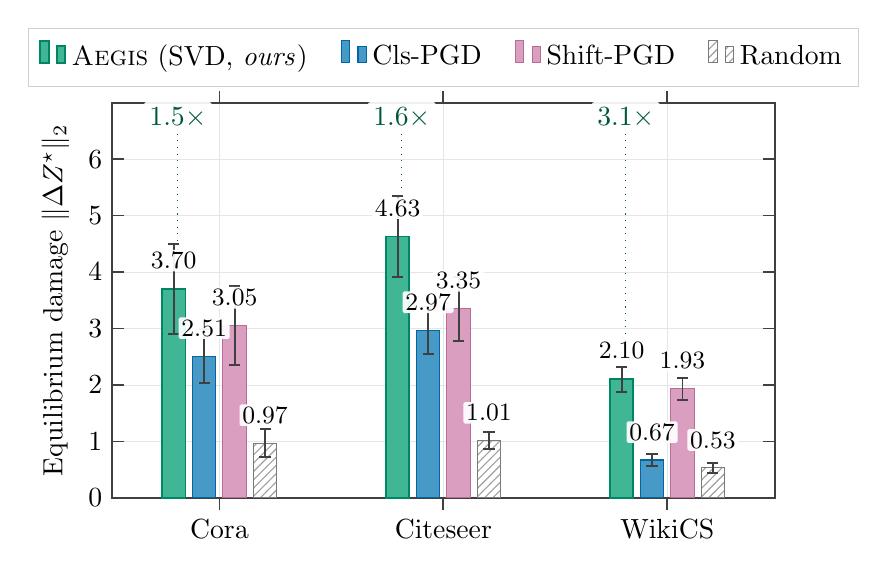
\begin{tikzpicture}[font=\rmfamily]
\begin{axis}[
    width=10.0cm, height=6.6cm,
    ybar=2.5pt,
    bar width=8.5pt,
    ymin=0, ymax=7.0,                 % headroom for value labels + gain tags
    enlarge x limits=0.24,
    ylabel={Equilibrium damage $\|\Delta Z^\star\|_2$},
    symbolic x coords={Cora, Citeseer, WikiCS},
    xtick=data,
    ytick={0,1,2,3,4,5,6},
    grid=major,
    grid style={line width=.25pt, draw=okGrey!22},
    axis line style={line width=0.6pt, draw=black!75},
    tick style={line width=0.6pt, draw=black!75},
    % Legend: 4 entries in a single horizontal row above the chart, just
    % under the title.
    legend style={
        at={(0.5,1.04)}, anchor=south,
        legend columns=4,
        font=\normalsize,
        draw=okGrey!40,
        line width=0.4pt,
        /tikz/every even column/.append style={column sep=10pt},
        inner sep=4pt,
    },
    legend cell align={left},
    tick label style={font=\normalsize},
    label style={font=\normalsize},
    % Per-bar value labels: positioned above the error-bar tip in serif 11pt
    % black. Two-decimal format matches tab:attack_full.
    nodes near coords,
    nodes near coords align={vertical},
    % All node-near-coord styling kept inside ONE block to avoid pgfkeys
    % context bleed from the trailing `/pgf/number format/.cd` switch.
    % Value labels: small serif font + white-fill bbox so the label sits
    % cleanly clear of the error-bar caps (yshift=6pt pushes the label
    % above the cap; the white bbox additionally masks the cap if any
    % vertical overlap remains for tight bars).
    nodes near coords style={
        font=\small, color=black, inner sep=1pt, yshift=6pt,
        fill=white, fill opacity=0.92, text opacity=1,
        rounded corners=0.6pt,
        /pgf/number format/.cd, fixed, fixed zerofill, precision=2,
    },
    error bars/error bar style={line width=0.7pt, color=black!75},
    error bars/error mark options={rotate=90, mark size=2.0pt, line width=0.7pt},
    clip=false,
]
% AEGIS (SVD) -- mean +/- std at eps = 0.10 from tab:attack_full
% Slightly thicker border (0.7pt vs 0.4pt) highlights "our method".
\addplot+[fill=okGreen!75, draw=okGreen!85!black, line width=0.7pt,
    error bars/.cd, y dir=both, y explicit]
    coordinates {
        (Cora,3.70)     +- (0,0.79)
        (Citeseer,4.63) +- (0,0.71)
        (WikiCS,2.10)   +- (0,0.22)
    };
\addlegendentry{\AEGIS (SVD, \emph{ours})}

% Cls-PGD
\addplot+[fill=okBlue!72, draw=okBlue!90!black, line width=0.4pt,
    error bars/.cd, y dir=both, y explicit]
    coordinates {
        (Cora,2.51)     +- (0,0.48)
        (Citeseer,2.97) +- (0,0.42)
        (WikiCS,0.67)   +- (0,0.11)
    };
\addlegendentry{Cls-PGD}

% Shift-PGD
\addplot+[fill=okPink!72, draw=okPink!90!black, line width=0.4pt,
    error bars/.cd, y dir=both, y explicit]
    coordinates {
        (Cora,3.05)     +- (0,0.70)
        (Citeseer,3.35) +- (0,0.57)
        (WikiCS,1.93)   +- (0,0.20)
    };
\addlegendentry{Shift-PGD}

% Random
\addplot+[fill=okGrey!40, draw=okGrey!90!black, line width=0.4pt,
    pattern=north east lines, pattern color=okGrey!80,
    error bars/.cd, y dir=both, y explicit]
    coordinates {
        (Cora,0.97)     +- (0,0.25)
        (Citeseer,1.01) +- (0,0.15)
        (WikiCS,0.53)   +- (0,0.09)
    };
\addlegendentry{Random}

% --- AEGIS gain factor (over Cls-PGD) -----------------------------------
% Consistent format and CONSISTENT position above each AEGIS bar:
% gain = AEGIS_mean / Cls-PGD_mean
%   Cora:     3.70 / 2.51 = 1.5x
%   Citeseer: 4.63 / 2.97 = 1.6x
%   WikiCS:   2.10 / 0.67 = 3.1x
% Each tag is placed near the top of the chart and connected to its AEGIS
% bar by a thin coloured leader. The leader makes the comparison target
% (AEGIS bar) unambiguous, and the constant y=6.5 keeps the three tags on
% a visual horizon for instant scanning.
% Leader and tag use okGreen!55!black so they match the AEGIS bar.
% NOTE: pgfplots' symbolic x axis snaps to category centres; we shift to
% the AEGIS bar (leftmost of the 4 within each group) using `xshift`.
\node[font=\normalsize\bfseries, color=okGreen!55!black, anchor=south,
      fill=white, fill opacity=0.92, text opacity=1, inner sep=2pt,
      rounded corners=1pt]
     (gCora) at ([xshift=-15pt]axis cs:Cora, 6.45)
     {$1.5\times$};
\node[font=\normalsize\bfseries, color=okGreen!55!black, anchor=south,
      fill=white, fill opacity=0.92, text opacity=1, inner sep=2pt,
      rounded corners=1pt]
     (gCite) at ([xshift=-15pt]axis cs:Citeseer, 6.45)
     {$1.6\times$};
\node[font=\normalsize\bfseries, color=okGreen!55!black, anchor=south,
      fill=white, fill opacity=0.92, text opacity=1, inner sep=2pt,
      rounded corners=1pt]
     (gWiki) at ([xshift=-15pt]axis cs:WikiCS, 6.45)
     {$3.1\times$};
% Thin colour-matched leader from each gain tag down to the AEGIS bar top
\draw[okGreen!55!black, line width=0.4pt, dotted]
    (gCora.south) -- ([xshift=-15pt]axis cs:Cora, 4.55);
\draw[okGreen!55!black, line width=0.4pt, dotted]
    (gCite.south) -- ([xshift=-15pt]axis cs:Citeseer, 5.40);
\draw[okGreen!55!black, line width=0.4pt, dotted]
    (gWiki.south) -- ([xshift=-15pt]axis cs:WikiCS, 2.40);

% (Gain reference -- "$k\times$ over Cls-PGD" -- left to the figure caption
%  so the inline annotation row stays uncluttered.)

\end{axis}
\end{tikzpicture}
\end{document}
